
\uc{Creazione \textit{conversazione libera}\textsubscript{G}}{conv_libera}
\begin{itemize}
    \item \textbf{Attori coinvolti}: Installatore;
    \item \textbf{Descrizione}: L’installatore desidera interrogare il \textit{sistema}\textsubscript{G}, quindi crea una nuova \textit{conversazione libera}\textsubscript{G} per richiedere le informazioni a lui necessarie tramite domande poste in linguaggio naturale;
    \item \textbf{Precondizioni}: L’installatore ha accesso all’\textit{interfaccia web}\textsubscript{G} del \textit{sistema}\textsubscript{G};
    \item \textbf{Postcondizioni}: Il \textit{sistema}\textsubscript{G} crea una nuova \textit{conversazione libera}\textsubscript{G} a cui puó accedere l’installatore, dove potrà porre liberamente domande in linguaggio naturale al \textit{sistema}\textsubscript{G};
    \item \textbf{Scenario principale}:
    \begin{enumerate}
    \item L’installatore accede all’\textit{interfaccia web}\textsubscript{G} di Vimar GENIALE;
    \item Richiede la creazione di una nuova conversazione in modalità libera;
    \item Il \textit{sistema}\textsubscript{G} esegue la creazione della nuova conversazione nella modalità desiderata dall’utente;
    \item  L’installatore accede alla nuova conversazione.
    \end{enumerate}
    \item \textbf{Estensioni}: UC2 - Raggiungimento limite di conversazioni;
\end{itemize}
\begin{figure}[H]
\centering
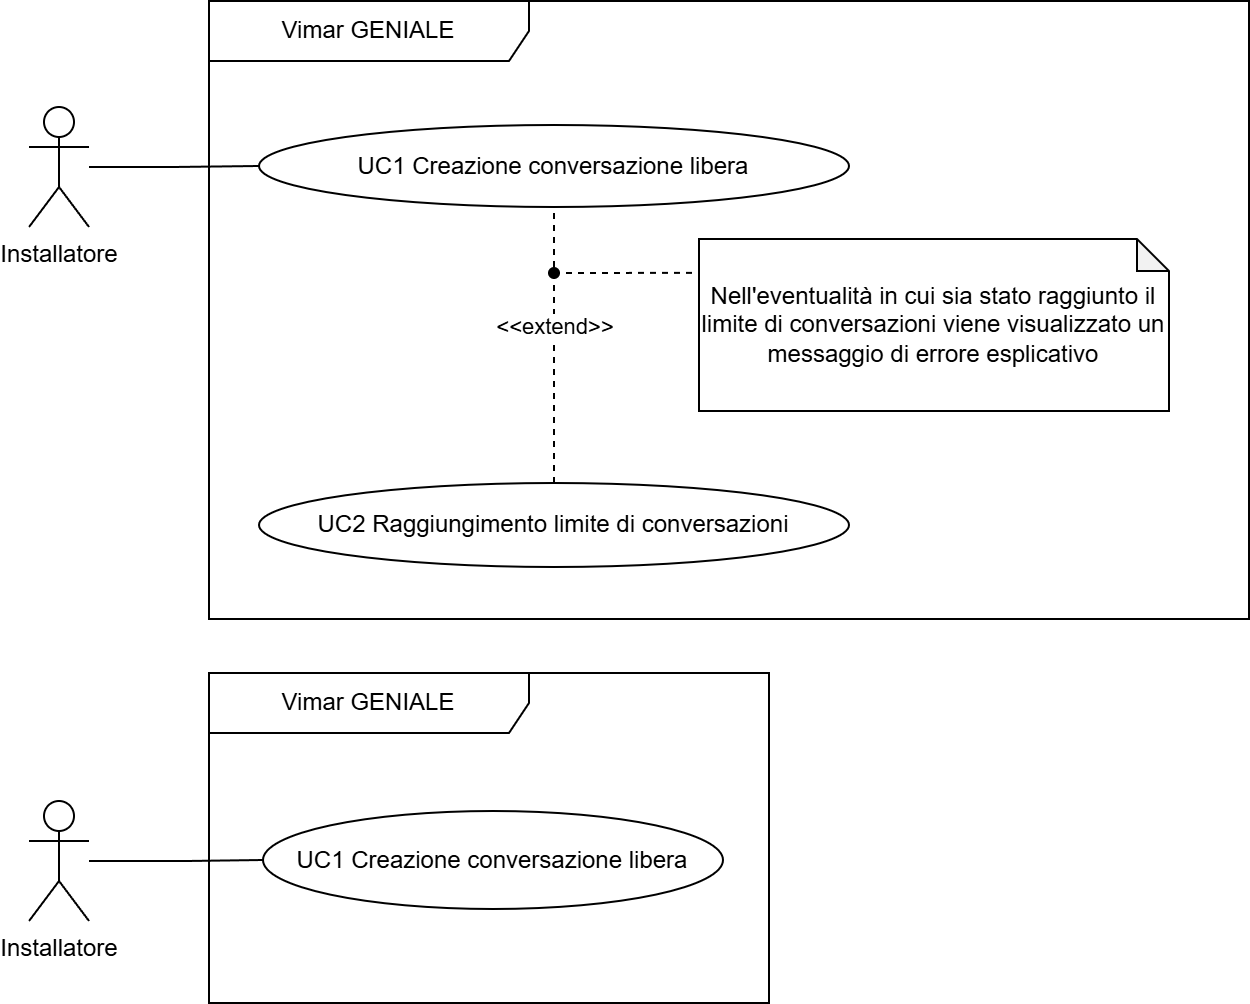
\includegraphics[width=0.8\textwidth]{contents/casi_duso/png/UC1.png}
\caption{UC1, UC2 - Creazione \textit{conversazione libera}\textsubscript{G}}
% \label{fig:UC1a}
\end{figure}

\uc{Raggiungimento limite di conversazioni}{limite_conv}
\begin{itemize}
    \item \textbf{Attori coinvolti}: Installatore;
    \item \textbf{Descrizione}: L’installatore desidera interrogare il \textit{sistema}\textsubscript{G}, ma quando prova a creare una nuova conversazione per richiedere le informazioni a lui necessarie, supera il limite massimo di conversazioni supportate;
    \item \textbf{Precondizioni}: 
        \begin{itemize}
            \item L’installatore ha accesso all’\textit{interfaccia web}\textsubscript{G} del \textit{sistema}\textsubscript{G};
            \item Il numero di conversazioni memorizzate nel \textit{sistema}\textsubscript{G} supera il limite massimo supportato;
        \end{itemize}
    \item \textbf{Postcondizioni}:  Il \textit{sistema}\textsubscript{G} restituisce una risposta che indica il motivo per cui si è verificato l’errore;
    \item \textbf{Scenario principale}:
    \begin{enumerate}
    \item L’installatore accede all’\textit{interfaccia web}\textsubscript{G} di Vimar GENIALE;
    \item Richiede la creazione di una nuova conversazione, nonostante siano già esistenti un numero di conversazioni che raggiunge il limite;
    \item Il \textit{sistema}\textsubscript{G} elabora la richiesta e fornisce una risposta che spiega la causa dell'errore riscontrato;
    \item L’installatore visualizza le informazioni sull’errore che si è verificato.
    \end{enumerate}
\end{itemize}



\uc{Salvataggio conversazione}{salvataggio_conv}
\begin{itemize}
    \item \textbf{Attori coinvolti}: Installatore;
    \item \textbf{Descrizione}: L’installatore, prima di chiudere l’applicativo, desidera salvare le conversazioni memorizzate attualmente all’interno del \textit{sistema}\textsubscript{G}, per poterle utilizzare nuovamente dal punto in cui ha concluso in precedenza alla prossima apertura dell’applicativo;
    \item \textbf{Precondizioni}: 
        \begin{itemize}
            \item L’installatore ha accesso all’\textit{interfaccia web}\textsubscript{G} del \textit{sistema}\textsubscript{G};
            \item Sono presenti nel \textit{sistema}\textsubscript{G} un numero consentito di conversazioni;
        \end{itemize}
    \item \textbf{Postcondizioni}: Il \textit{sistema}\textsubscript{G} salva le conversazioni memorizzate attualmente all’interno del \textit{sistema}\textsubscript{G};
    \item \textbf{Scenario principale}:
    \begin{enumerate}
    \item L’installatore accede all’\textit{interfaccia web}\textsubscript{G} di Vimar GENIALE;
    \item Richiede il salvataggio delle conversazioni esistenti al momento, prima di effettuare la chiusura dell’applicativo;
    \item Il \textit{sistema}\textsubscript{G} effettua il salvataggio e fornisce una risposta che conferma il completamento dell’operazione;
    \item L’installatore visualizza il messaggio di conferma dell’avvenuto salvataggio.
    \end{enumerate}
    \item \textbf{Estensioni}: UC4 - Salvataggio conversazione vuota
\end{itemize}
\begin{figure}[H]
\centering
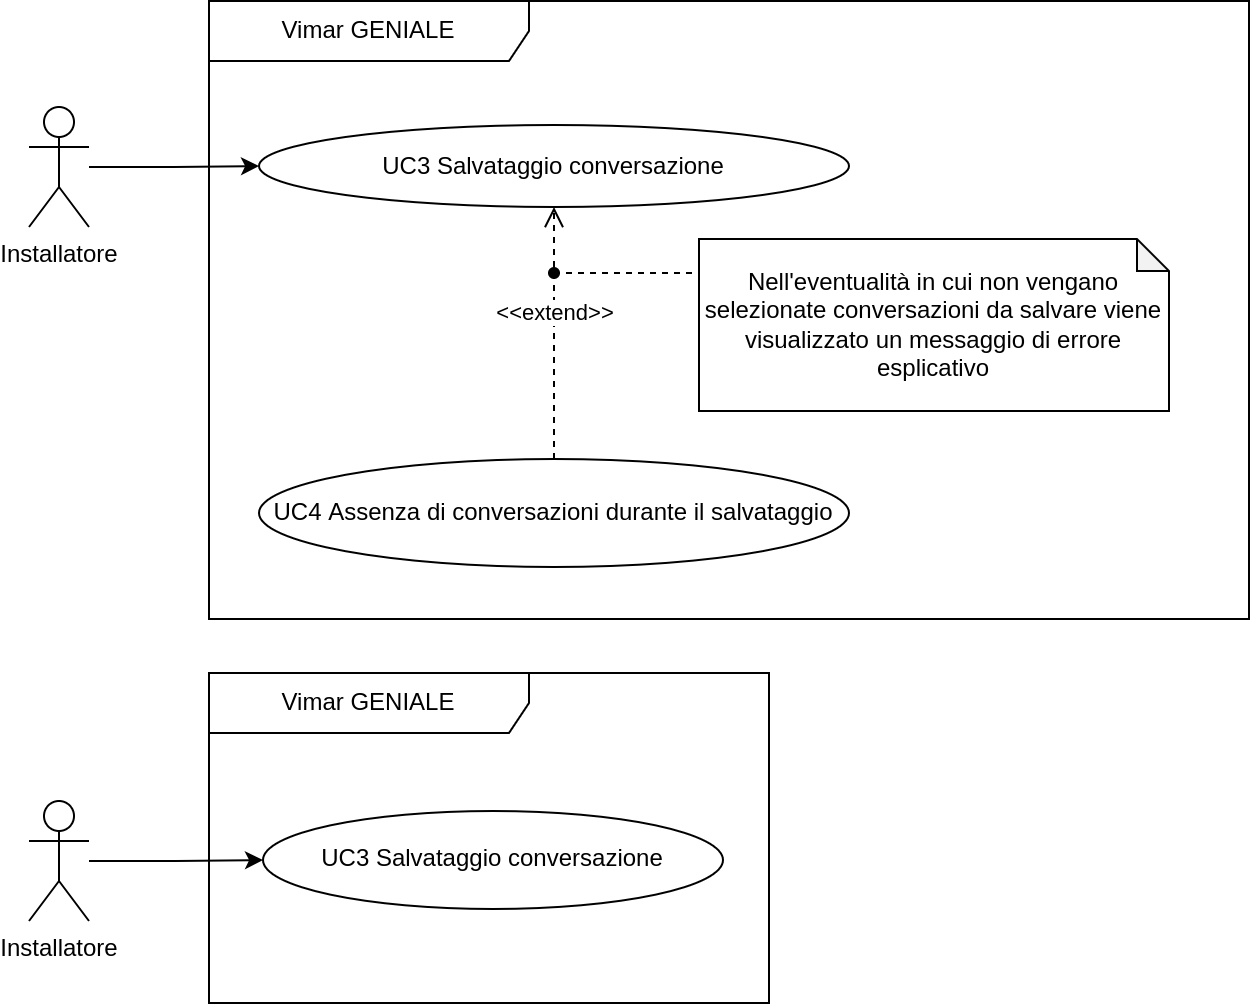
\includegraphics[width=0.8\textwidth]{contents/casi_duso/png/UC3.png}
\caption{UC3, UC4 - Salvataggio conversazione}
% \label{fig:UC1a}
\end{figure}

\uc{Salvataggio conversazione vuota}{assenza_conv}
\begin{itemize}
    \item \textbf{Attori coinvolti}: Installatore;
    \item \textbf{Descrizione}: L’installatore tenta di salvare una o più conversazioni vuote;
    \item \textbf{Precondizioni}: 
        \begin{itemize}
            \item L’installatore ha accesso all’\textit{interfaccia web}\textsubscript{G} del \textit{sistema}\textsubscript{G};
            \item L'installatore crea una nuova \textit{conversazione libera}\textsubscript{G} e poi non fa nessuna domanda.
        \end{itemize}
    \item \textbf{Postcondizioni}: Il \textit{sistema}\textsubscript{G} restituisce una risposta che indica il motivo per cui si è verificato l’errore;
    \item \textbf{Scenario principale}:
    \begin{enumerate}
    \item L’installatore accede all’\textit{interfaccia web}\textsubscript{G} di Vimar GENIALE;
    \item L'installatore crea una nuova conversazione, ma non pone nessuna domanda.
    \item Richiede il salvataggio di una o più conversazioni;
    \item Il \textit{sistema}\textsubscript{G} elabora la richiesta e fornisce una risposta che spiega la causa dell'errore riscontrato;
    \item L’installatore visualizza le informazioni sull’errore che si è verificato.
    \end{enumerate}
\end{itemize}



\uc{Cancellazione conversazione}{cancellazione_conv}
\begin{itemize}
    \item \textbf{Attori coinvolti}: Installatore;
    \item \textbf{Descrizione}: L’installatore desidera eliminare una conversazione esistente, in quanto non è ritenuta più necessaria al suo scopo;
    \item \textbf{Precondizioni}: 
        \begin{itemize}
            \item L’installatore ha accesso all’\textit{interfaccia web}\textsubscript{G} del \textit{sistema}\textsubscript{G};
            \item L’installatore ha accesso ad una conversazione memorizzata nel \textit{sistema}\textsubscript{G};
        \end{itemize}
    \item \textbf{Postcondizioni}: Il \textit{sistema}\textsubscript{G} elimina la conversazione non ritenuta più necessaria dall’installatore.
    \item \textbf{Scenario principale}:
    \begin{enumerate}
    \item L’installatore accede all’\textit{interfaccia web}\textsubscript{G} di Vimar GENIALE;
    \item Richiede l’eliminazione di una conversazione, in quanto ha raggiunto il suo scopo e non è più utile;
    \item Il \textit{sistema}\textsubscript{G} effettua l’eliminazione e fornisce una risposta che conferma il completamento dell’operazione;
    \item L’installatore visualizza il messaggio di conferma dell’avvenuta cancellazione.
    \end{enumerate}
\end{itemize}
\begin{figure}[H]
\centering
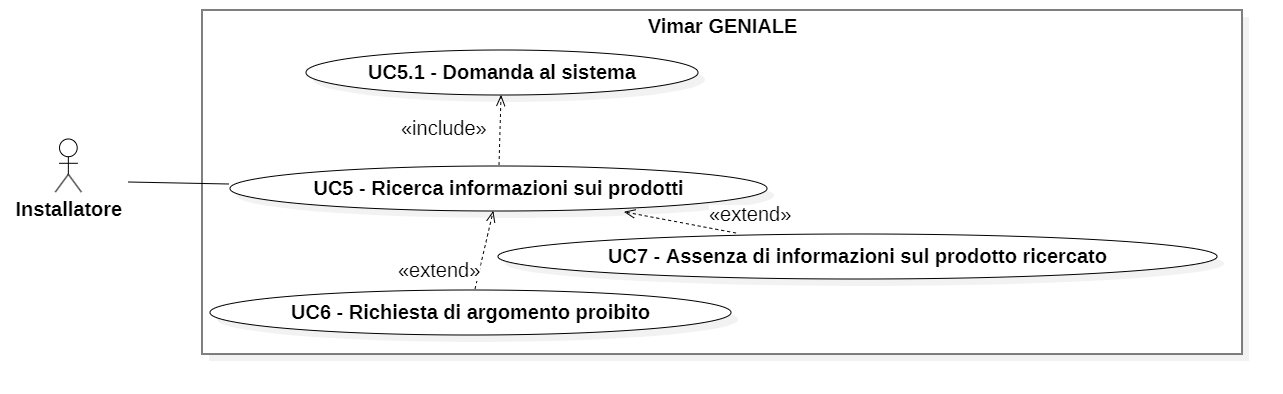
\includegraphics[width=0.8\textwidth]{contents/casi_duso/png/UC5.png}
\caption{UC5 - Cancellazione conversazione}
% \label{fig:UC1a}
\end{figure}


\uc{Ricerca informazioni sui prodotti con \textit{conversazione libera}\textsubscript{G}}{ricerca_info_prodotti}
\begin{itemize}
    \item \textbf{Attori coinvolti}: Installatore;
    \item \textbf{Descrizione}: L’installatore interroga il \textit{sistema}\textsubscript{G} per ottenere informazioni dettagliate su un prodotto specifico, come schemi elettrici, dati tecnici e manuali;
    \item \textbf{Precondizioni}: 
        \begin{itemize}
            \item L’installatore ha accesso all’\textit{interfaccia web}\textsubscript{G} del \textit{sistema}\textsubscript{G};
            \item L’installatore ha accesso ad una conversazione memorizzabile nel \textit{sistema}\textsubscript{G};
            \item Il prodotto richiesto è registrato nel \textit{sistema}\textsubscript{G} e le informazioni sono correttamente indicizzate.
        \end{itemize}
    \item \textbf{Postcondizioni}: Il \textit{sistema}\textsubscript{G} restituisce le informazioni richieste, incluse le descrizioni del prodotto, schemi elettrici e manuali di configurazione;
    \item \textbf{Scenario principale}:
    \begin{enumerate}
    \item L’installatore accede all’\textit{interfaccia web}\textsubscript{G} di Vimar GENIALE;
    \item Inserisce una domanda o una parola chiave relativa ad un prodotto specifico;
    \item Il \textit{sistema}\textsubscript{G} esegue la ricerca nel \textit{database}\textsubscript{G} le informazioni necessarie a fornire sufficiente contesto al \textit{LLM}\textsubscript{G}.
    \end{enumerate}
    \item \textbf{Inclusioni}: UC18 - Digitare la domanda.
    \item \textbf{Estensioni}: 
    \begin{itemize}
        \item UC8 - Assenza di informazioni sul prodotto ricercato;
        \item UC15 - Richiesta di argomento proibito
    \end{itemize}

\end{itemize}
\begin{figure}[H]
\centering
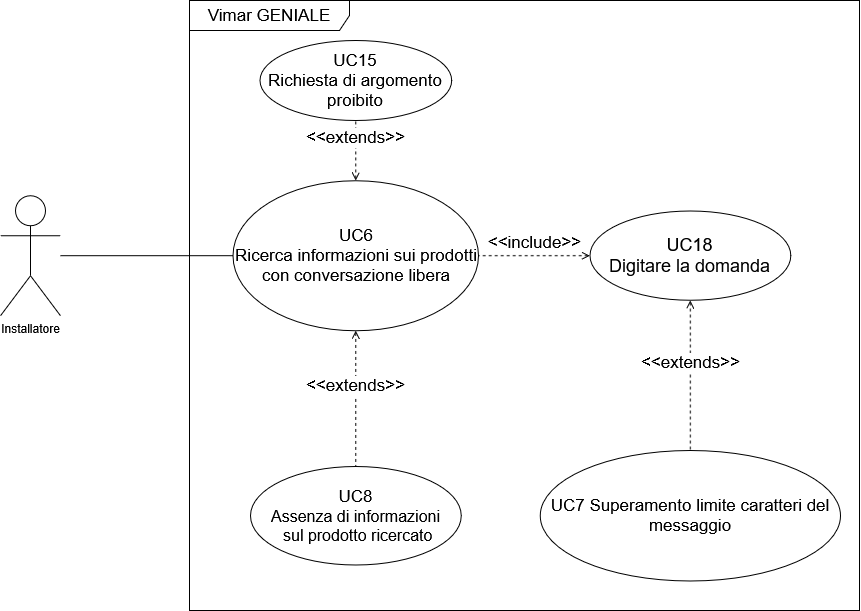
\includegraphics[width=0.8\textwidth]{contents/casi_duso/png/UC6.png}
\caption{UC6, UC7, UC8, UC15, UC16, UC18 - Ricerca informazioni sui prodotti con \textit{conversazione libera}\textsubscript{G}}
\end{figure}


\uc{Superamento limite caratteri del messaggio}{superamento_limite_caratteri}
\begin{itemize}
    \item \textbf{Attori coinvolti}: Installatore;
    \item \textbf{Descrizione}: L’installatore, quando interroga il \textit{sistema}\textsubscript{G} per ottenere informazioni, supera il limite di caratteri che possono essere utilizzati per effettuare la richiesta;
    \item \textbf{Precondizioni}: 
        \begin{itemize}
            \item L’installatore ha accesso all’\textit{interfaccia web}\textsubscript{G} del \textit{sistema}\textsubscript{G};
            \item L’installatore ha accesso ad una conversazione memorizzabile nel \textit{sistema}\textsubscript{G};
            \item La domanda posta supera il limite massimo di caratteri consentiti.
        \end{itemize}
    \item \textbf{Postcondizioni}: Il \textit{sistema}\textsubscript{G} restituisce una risposta che indica il motivo per cui si è verificato l’errore;
    \item \textbf{Scenario principale}:
    \begin{enumerate}
    \item L’installatore accede all’\textit{interfaccia web}\textsubscript{G} di Vimar GENIALE;
    \item Inserisce una domanda o una parola chiave relativa ad un prodotto specifico, superando il limite massimo consentito di caratteri;
    \item Il \textit{sistema}\textsubscript{G} elabora la richiesta e fornisce una risposta che spiega la causa dell'errore riscontrato;
    \item L’installatore visualizza le informazioni sull’errore che si è verificato.
    \end{enumerate}
\end{itemize}


\uc{Assenza di informazioni sul prodotto ricercato}{assenza_info_prodotto}
\begin{itemize}
    \item \textbf{Attori coinvolti}: Installatore;
    \item \textbf{Descrizione}: L’installatore interroga il \textit{sistema}\textsubscript{G} per ottenere informazioni dettagliate su un prodotto specifico, ma il \textit{sistema}\textsubscript{G} non è in grado di trovare nessuna informazione relativa ad esso;
    \item \textbf{Precondizioni}: 
        \begin{itemize}
            \item L’installatore ha accesso all’\textit{interfaccia web}\textsubscript{G} del \textit{sistema}\textsubscript{G};
            \item L’installatore ha accesso ad una conversazione memorizzabile nel \textit{sistema}\textsubscript{G};
            \item L’installatore pone una domanda al \textit{sistema}\textsubscript{G};
            \item Il \textit{sistema}\textsubscript{G} non è in possesso di alcuna informazione relativa al prodotto ricercato.
        \end{itemize}
    \item \textbf{Postcondizioni}: Il \textit{sistema}\textsubscript{G} restituisce una risposta che indica il motivo per cui si è verificato l’errore;
    \item \textbf{Scenario principale}:
    \begin{enumerate}
    \item L’installatore accede all’\textit{interfaccia web}\textsubscript{G} di Vimar GENIALE;
    \item Inserisce una domanda o una parola chiave relativa ad un prodotto specifico;
    \item Il \textit{sistema}\textsubscript{G} elabora la richiesta e fornisce una risposta che spiega la causa dell'errore riscontrato;
    \item L’installatore visualizza le informazioni sull’errore che si è verificato.
    \end{enumerate}
\end{itemize}


\uc{Visualizzazione storico dei messaggi}{visualizzazione_storico_messaggi}
\begin{itemize}
    \item \textbf{Attori coinvolti}: Installatore;
    \item \textbf{Descrizione}: L’installatore, avendo la necessità di riesaminare le risposte ricevute alle domande poste in precedenza, richiede al \textit{sistema}\textsubscript{G} di mostrare uno storico dei messaggi della conversazione attuale;
    \item \textbf{Precondizioni}: 
        \begin{itemize}
            \item L’installatore ha accesso all’\textit{interfaccia web}\textsubscript{G} del \textit{sistema}\textsubscript{G};
            \item L’installatore ha accesso ad una conversazione memorizzabile nel \textit{sistema}\textsubscript{G};
            \item La conversazione attuale contiene dei messaggi che sono stati scambiati in precedenza.
        \end{itemize}
    \item \textbf{Postcondizioni}: Il \textit{sistema}\textsubscript{G} ritorna lo storico dei messaggi della conversazione attuale.
    \item \textbf{Scenario principale}:
    \begin{enumerate}
    \item L’installatore accede all’\textit{interfaccia web}\textsubscript{G} di Vimar GENIALE;
    \item Accede ad una conversazione presente nel \textit{sistema}\textsubscript{G} e richiede di visualizzarne uno storico dei messaggi;
    \item Il \textit{sistema}\textsubscript{G} elabora la richiesta e fornisce lo storico dei messaggi della conversazione attuale;
    \item L’installatore visualizza i messaggi scambiati in precedenza nella conversazione corrente.
    \end{enumerate}
    \item \textbf{Estensioni}: UC10 - Mancanza messaggi pregressi nella conversazione
\end{itemize}
\begin{figure}[H]
\centering
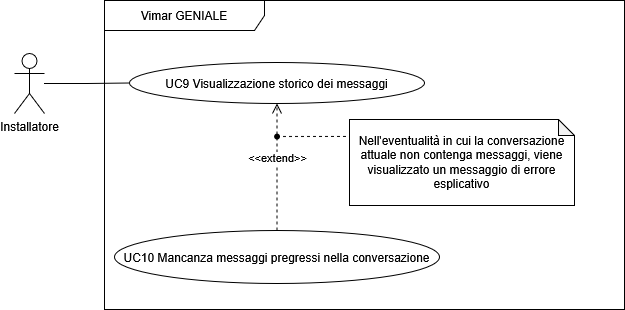
\includegraphics[width=0.8\textwidth]{contents/casi_duso/png/UC9.png}
\caption{UC9, UC10 - Visualizzazione storico dei messaggi}
% \label{fig:UC1a}
\end{figure}

\uc{Mancanza messaggi pregressi nella conversazione}{mancanza_messaggi_pregressi}
\begin{itemize}
    \item \textbf{Attori coinvolti}: Installatore;
    \item \textbf{Descrizione}: L’installatore richiede di visualizzare lo storico dei messaggi di una conversazione, ma non ci sono messaggi pregressi nella conversazione attuale;
    \item \textbf{Precondizioni}: 
        \begin{itemize}
            \item L’installatore ha accesso all’\textit{interfaccia web}\textsubscript{G} del \textit{sistema}\textsubscript{G};
            \item L’installatore ha accesso ad una conversazione memorizzabile nel \textit{sistema}\textsubscript{G};
            \item La conversazione attuale non contiene messaggi scambiati in precedenza.
        \end{itemize}
    \item \textbf{Postcondizioni}: Il \textit{sistema}\textsubscript{G} restituisce una risposta che indica l’assenza di messaggi pregressi nella conversazione attuale;
    \item \textbf{Scenario principale}:
    \begin{enumerate}
    \item L’installatore accede all’\textit{interfaccia web}\textsubscript{G} di Vimar GENIALE;
    \item Accede ad una conversazione presente nel \textit{sistema}\textsubscript{G} e richiede di visualizzarne uno storico dei messaggi;
    \item Il \textit{sistema}\textsubscript{G} elabora la richiesta e fornisce una risposta che indica l’assenza di messaggi pregressi nella conversazione attuale;
    \item L’installatore visualizza il messaggio che indica l’assenza di messaggi pregressi.
    \end{enumerate}
\end{itemize}



\uc{Fornitura di \textit{feedback}\textsubscript{G} sulla risposta del \textit{sistema}\textsubscript{G} ad interrogazione}{fornitura_feedback}
\begin{itemize}
    \item \textbf{Attori coinvolti}: Installatore;
    \item \textbf{Descrizione}: L’installatore, a seguito dell’interrogazione del \textit{sistema}\textsubscript{G} per ottenere informazioni, desidera fornire un \textit{feedback}\textsubscript{G} che indichi se la risposta ricevuta sia corretta o meno;
    \item \textbf{Precondizioni}: 
        \begin{itemize}
            \item L’installatore ha accesso all’\textit{interfaccia web}\textsubscript{G} del \textit{sistema}\textsubscript{G};
            \item L’installatore ha accesso ad una conversazione memorizzabile nel \textit{sistema}\textsubscript{G};
            \item Il \textit{sistema}\textsubscript{G} fornisce una risposta ad un’interrogazione da parte dell’installatore.
        \end{itemize}
    \item \textbf{Postcondizioni}: L’installatore, dopo aver esaminato la risposta ricevuta, fornisce un riscontro sulla correttezza di quest’ultima che verrà registrato dal \textit{sistema}\textsubscript{G};
    \item \textbf{Scenario principale}:
    \begin{enumerate}
    \item L’installatore accede all’\textit{interfaccia web}\textsubscript{G} di Vimar GENIALE;
    \item Inserisce una domanda o una parola chiave relativa ad un prodotto specifico;
    \item Il \textit{sistema}\textsubscript{G} esegue la ricerca nel \textit{database}\textsubscript{G} dei prodotti e restituisce una risposta che include informazioni dettagliate come schemi, descrizioni e manuali;
    \item L’installatore visualizza le informazioni fornite e, dopo aver verificato la correttezza delle informazioni ricevute, fornisce un \textit{feedback}\textsubscript{G} sulla risposta al \textit{sistema}\textsubscript{G};
    \item Il \textit{sistema}\textsubscript{G} registra il \textit{feedback}\textsubscript{G} ricevuto dall’installatore.
    \end{enumerate}
\end{itemize}
\begin{figure}[H]
\centering
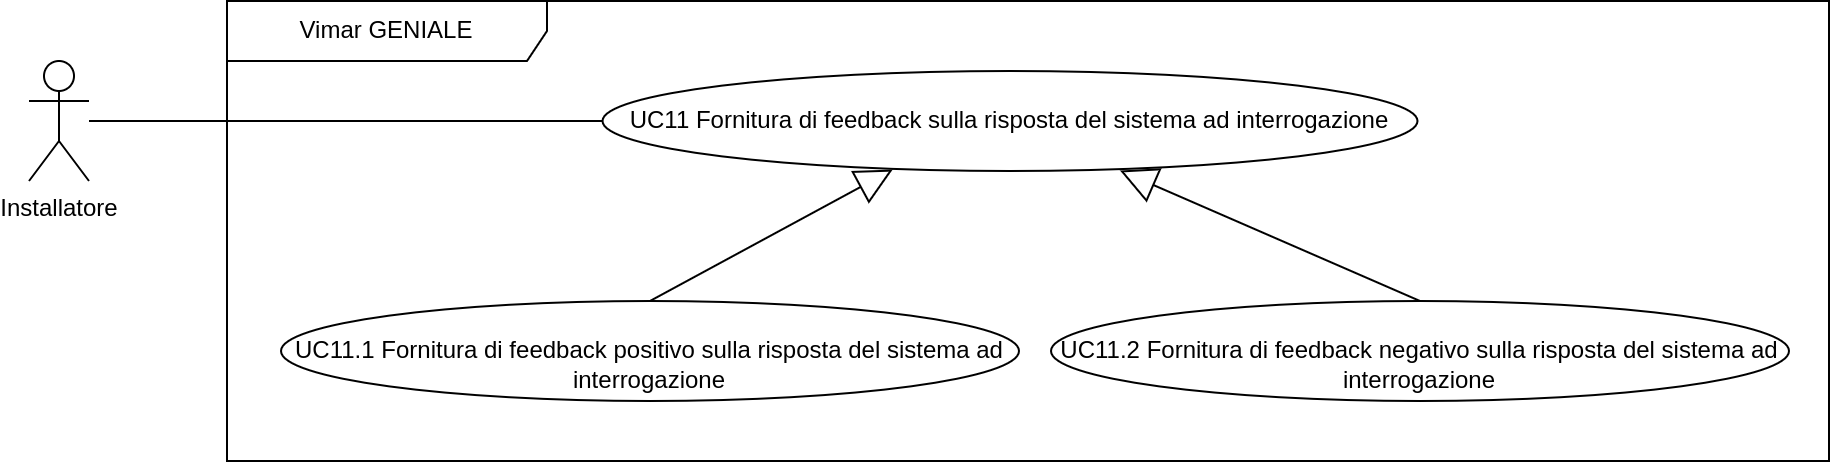
\includegraphics[width=0.8\textwidth]{contents/casi_duso/png/UC11.png}
\caption{UC11, UC11.1, UC11.2 - Fornitura di \textit{feedback}\textsubscript{G} sulla risposta del \textit{sistema}\textsubscript{G} ad interrogazione}
% \label{fig:UC1a}
\end{figure}

\subuc{Fornitura di \textit{feedback}\textsubscript{G} positivo sulla risposta del \textit{sistema}\textsubscript{G} ad interrogazione}{feedback_positivo}
\begin{itemize}
    \item \textbf{Attori coinvolti}: Installatore;
    \item \textbf{Descrizione}: L’installatore, a seguito dell’interrogazione del \textit{sistema}\textsubscript{G} per ottenere informazioni, desidera fornire un \textit{feedback}\textsubscript{G} che indichi che la risposta ricevuta è corretta;
    \item \textbf{Precondizioni}: 
        \begin{itemize}
            \item L’installatore ha accesso all’\textit{interfaccia web}\textsubscript{G} del \textit{sistema}\textsubscript{G};
            \item L’installatore ha accesso ad una conversazione memorizzata nel \textit{sistema}\textsubscript{G};
            \item Il \textit{sistema}\textsubscript{G} fornisce una risposta corretta ad un’interrogazione da parte dell’installatore.
        \end{itemize}
    \item \textbf{Postcondizioni}: L’installatore, dopo aver esaminato la risposta ricevuta, fornisce un riscontro positivo sulla correttezza di quest’ultima che verrà registrato dal \textit{sistema}\textsubscript{G};
    \item \textbf{Scenario principale}:
    \begin{enumerate}
    \item L’installatore accede all’\textit{interfaccia web}\textsubscript{G} di Vimar GENIALE;
    \item Inserisce una domanda o una parola chiave relativa ad un prodotto specifico;
    \item Il \textit{sistema}\textsubscript{G} esegue la ricerca nel \textit{database}\textsubscript{G} dei prodotti e restituisce una risposta che include informazioni dettagliate come schemi, descrizioni e manuali;
    \item L’installatore visualizza le informazioni fornite e, dopo aver verificato la correttezza delle informazioni ricevute, fornisce un \textit{feedback}\textsubscript{G} positivo sulla risposta al \textit{sistema}\textsubscript{G};
    \item Il \textit{sistema}\textsubscript{G} registra il \textit{feedback}\textsubscript{G} ricevuto dall’installatore.
    \end{enumerate}
    \item \textbf{Generalizzazioni}: UC11 - Fornitura di feedback$_G$ sulla risposta del sistema ad interrogazione.
\end{itemize}

\subuc{Fornitura di \textit{feedback}\textsubscript{G} negativo sulla risposta del \textit{sistema}\textsubscript{G} ad interrogazione}{feedback_negativo}
\begin{itemize}
    \item \textbf{Attori coinvolti}: Installatore;
    \item \textbf{Descrizione}: L’installatore, a seguito dell’interrogazione del \textit{sistema}\textsubscript{G} per ottenere informazioni, desidera fornire un \textit{feedback}\textsubscript{G} che indichi che la risposta ricevuta è errata;
    \item \textbf{Precondizioni}: 
        \begin{itemize}
            \item L’installatore ha accesso all’\textit{interfaccia web}\textsubscript{G} del \textit{sistema}\textsubscript{G};
            \item L’installatore ha accesso ad una conversazione memorizzata nel \textit{sistema}\textsubscript{G};
            \item Il \textit{sistema}\textsubscript{G} fornisce una risposta errata ad un’interrogazione da parte dell’installatore.
        \end{itemize}
    \item \textbf{Postcondizioni}: L’installatore, dopo aver esaminato la risposta ricevuta, fornisce un riscontro negativo sulla correttezza di quest’ultima che verrà registrato dal \textit{sistema}\textsubscript{G};
    \item \textbf{Scenario principale}:
    \begin{enumerate}
    \item L’installatore accede all’\textit{interfaccia web}\textsubscript{G} di Vimar GENIALE;
    \item Inserisce una domanda o una parola chiave relativa ad un prodotto specifico;
    \item Il \textit{sistema}\textsubscript{G} esegue la ricerca nel \textit{database}\textsubscript{G} dei prodotti e restituisce una risposta che include informazioni dettagliate come schemi, descrizioni e manuali;
    \item L’installatore visualizza le informazioni fornite e, dopo aver verificato la correttezza delle informazioni ricevute, fornisce un \textit{feedback}\textsubscript{G} negativo sulla risposta al \textit{sistema}\textsubscript{G};
    \item Il \textit{sistema}\textsubscript{G} registra il \textit{feedback}\textsubscript{G} ricevuto dall’installatore.
    \end{enumerate}
    \item \textbf{Generalizzazioni}: UC11 - Fornitura di feedback$_G$ sulla risposta del sistema ad interrogazione.

\end{itemize}

\uc{Accesso al \textit{cruscotto informativo}\textsubscript{G}}{accesso_cruscotto}
\begin{itemize}
    \item \textbf{Attori coinvolti}: \textit{Amministratore}\textsubscript{G};
    \item \textbf{Descrizione}: Un \textit{amministratore}\textsubscript{G} desidera accedere al \textit{cruscotto informativo}\textsubscript{G} per visualizzare una panoramica di informazioni relative all’utilizzo del \textit{sistema}\textsubscript{G};
    \item \textbf{Precondizioni}: 
        \begin{itemize}
            \item L’\textit{amministratore}\textsubscript{G} ha accesso all’\textit{interfaccia web}\textsubscript{G} del \textit{sistema}\textsubscript{G};
            \item L’\textit{amministratore}\textsubscript{G} è dotato delle credenziali necessarie ad accedere alla \textit{dashboard}\textsubscript{G}.
        \end{itemize}
    \item \textbf{Postcondizioni}: L’\textit{amministratore}\textsubscript{G} accede al \textit{cruscotto informativo}\textsubscript{G}, da cui può visualizzare svariate informazioni riguardanti l’uso del \textit{sistema}\textsubscript{G};
    \item \textbf{Scenario principale}:
    \begin{enumerate}
    \item L’\textit{amministratore}\textsubscript{G} accede all’\textit{interfaccia web}\textsubscript{G} di Vimar GENIALE;
    \item Inserisce le proprie credenziali;
    \item Il \textit{sistema}\textsubscript{G} riceve la richiesta di accesso e \textit{verifica}\textsubscript{G} le credenziali;
    \item L’\textit{amministratore}\textsubscript{G} ottiene l’accesso alla \textit{dashboard}\textsubscript{G}.
    \end{enumerate}
    \item \textbf{Estensioni}: UC13 - Inserimento \textit{username}\textsubscript{G} o \textit{password}\textsubscript{G} errati
    \item \textbf{Inclusioni}: UC12.1 - Inserimento \textit{username}\textsubscript{G} e \textit{password}\textsubscript{G}
\end{itemize}

\begin{figure}[H]
\centering
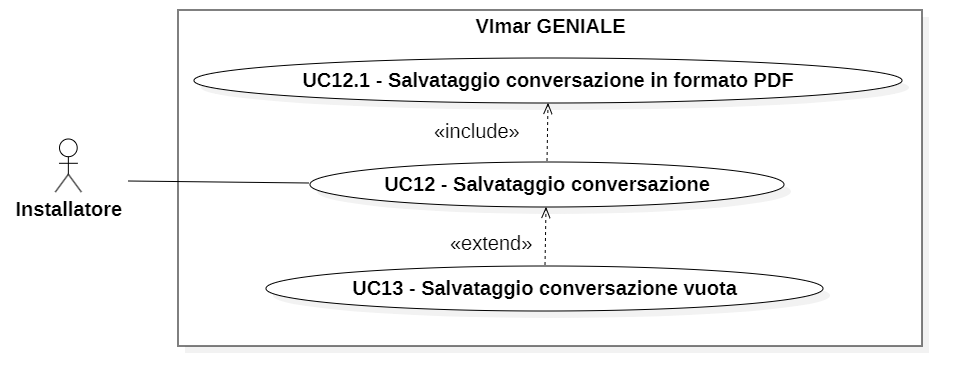
\includegraphics[width=0.8\textwidth]{contents/casi_duso/png/UC12.png}
\caption{UC12, UC12.1 UC13 - Accesso al \textit{cruscotto informativo}\textsubscript{G} }
% \label{fig:UC1a}
\end{figure}

\subuc{Inserimento \textit{username}\textsubscript{G} e \textit{password}\textsubscript{G}}{inserimento_username}
\begin{itemize}
    \item \textbf{Attori coinvolti}: \textit{Amministratore}\textsubscript{G};
    \item \textbf{Descrizione}: Un \textit{amministratore}\textsubscript{G} desidera accedere al \textit{cruscotto informativo}\textsubscript{G} per visualizzare una panoramica di informazioni relative all’utilizzo del \textit{sistema}\textsubscript{G}, dunque inserisce lo \textit{username}\textsubscript{G} e la \textit{password}\textsubscript{G};
    \item \textbf{Precondizioni}: 
        \begin{itemize}
            \item L’\textit{amministratore}\textsubscript{G} ha accesso all’\textit{interfaccia web}\textsubscript{G} del \textit{sistema}\textsubscript{G};
            \item L’\textit{amministratore}\textsubscript{G} è dotato dello \textit{username}\textsubscript{G} e della \textit{password}\textsubscript{G} necessarie ad accedere alla \textit{dashboard}\textsubscript{G}.
        \end{itemize}
    \item \textbf{Postcondizioni}: L’\textit{amministratore}\textsubscript{G} ha inserito lo \textit{username}\textsubscript{G} e la \textit{password}\textsubscript{G}, ovvero le credenziali richieste per l’accesso al \textit{cruscotto informativo}\textsubscript{G};
    \item \textbf{Scenario principale}:
    \begin{enumerate}
    \item L’\textit{amministratore}\textsubscript{G} accede all’\textit{interfaccia web}\textsubscript{G} di Vimar GENIALE;
    \item Inserisce lo \textit{username}\textsubscript{G}.
    \item Inserisce la \textit{password}\textsubscript{G}.
    \end{enumerate}
\end{itemize}


\uc{Inserimento \textit{username}\textsubscript{G} o \textit{password}\textsubscript{G} errati}{inserimento_cred_errati}
\begin{itemize}
    \item \textbf{Attori coinvolti}: \textit{Amministratore}\textsubscript{G};
    \item \textbf{Descrizione}: Un \textit{amministratore}\textsubscript{G} desidera accedere al \textit{cruscotto informativo}\textsubscript{G} per visualizzare una panoramica di informazioni relative all’utilizzo del \textit{sistema}\textsubscript{G}, ma non riesce ad accedere a causa di un errore nell’inserimento dello \textit{username}\textsubscript{G} o della \textit{password}\textsubscript{G};
    \item \textbf{Precondizioni}: 
        \begin{itemize}
            \item L’\textit{amministratore}\textsubscript{G} ha accesso all’\textit{interfaccia web}\textsubscript{G} del \textit{sistema}\textsubscript{G};
            \item L’\textit{amministratore}\textsubscript{G} è dotato delle credenziali necessarie ad accedere alla \textit{dashboard}\textsubscript{G};
            \item Lo \textit{username}\textsubscript{G} o la \textit{password}\textsubscript{G} non sono corretti.
        \end{itemize}
    \item \textbf{Postcondizioni}: Il \textit{sistema}\textsubscript{G} restituisce una risposta che indica il motivo per cui si è verificato l’errore;
    \item \textbf{Scenario principale}:
    \begin{enumerate}
    \item L’\textit{amministratore}\textsubscript{G} accede all’\textit{interfaccia web}\textsubscript{G} di Vimar GENIALE;
    \item Inserisce le proprie credenziali;
    \item Il \textit{sistema}\textsubscript{G} elabora la richiesta e fornisce una risposta che spiega l’inserimento errato delle credenziali;
    \item L’\textit{amministratore}\textsubscript{G} visualizza le informazioni sull’errore che si è verificato.
    \end{enumerate}
\end{itemize}

\uc{Visualizzazione informazioni sulla \textit{dashboard}\textsubscript{G}}{visualizzazione_info_dashboard}
\begin{itemize}
    \item \textbf{Attori coinvolti}: \textit{Amministratore}\textsubscript{G};
    \item \textbf{Descrizione}: Un \textit{amministratore}\textsubscript{G} desidera visualizzare una panoramica di informazioni relative all’utilizzo del \textit{sistema}\textsubscript{G} dal \textit{cruscotto informativo}\textsubscript{G};
    \item \textbf{Precondizioni}: 
        \begin{itemize}
            \item L’\textit{amministratore}\textsubscript{G} ha accesso all’\textit{interfaccia web}\textsubscript{G} del \textit{sistema}\textsubscript{G};
            \item L’\textit{amministratore}\textsubscript{G} è dotato dell’accesso alla \textit{dashboard}\textsubscript{G};
        \end{itemize}
    \item \textbf{Postcondizioni}: Il \textit{sistema}\textsubscript{G} raccoglie le informazioni richieste e le mostra nella \textit{dashboard}\textsubscript{G};
    \item \textbf{Scenario principale}:
    \begin{enumerate}
    \item L’\textit{amministratore}\textsubscript{G} accede all’\textit{interfaccia web}\textsubscript{G} di Vimar GENIALE;
    \item Inserisce le proprie credenziali;
    \item Il \textit{sistema}\textsubscript{G} riceve la richiesta di accesso e \textit{verifica}\textsubscript{G} le credenziali;
    \item L’\textit{amministratore}\textsubscript{G} ottiene l’accesso alla \textit{dashboard}\textsubscript{G};
    \item Il \textit{sistema}\textsubscript{G} mostra le informazioni richieste sul \textit{cruscotto informativo}\textsubscript{G}.
    \end{enumerate}
    \item \textbf{Inclusioni}: 
    \begin{itemize}
        \item UC12 - Accesso al \textit{cruscotto informativo}\textsubscript{G};
        \item UC14.1 - Visualizzazione numero richieste con \textit{conversazione libera}\textsubscript{G};
        \item UC14.2 - Visualizzazione numero richieste con \textit{conversazione guidata}\textsubscript{G};
        \item UC14.3 - Visualizzazione classifica di parole più utilizzate;
        \item UC14.4 - Visualizzazione numero risposte positive dal \textit{sistema}\textsubscript{G} di \textit{feedback}\textsubscript{G};
        \item UC14.5 - Visualizzazione numero negative positive dal \textit{sistema}\textsubscript{G} di \textit{feedback}\textsubscript{G}.
    \end{itemize}
\end{itemize}
\begin{figure}[H]
\centering
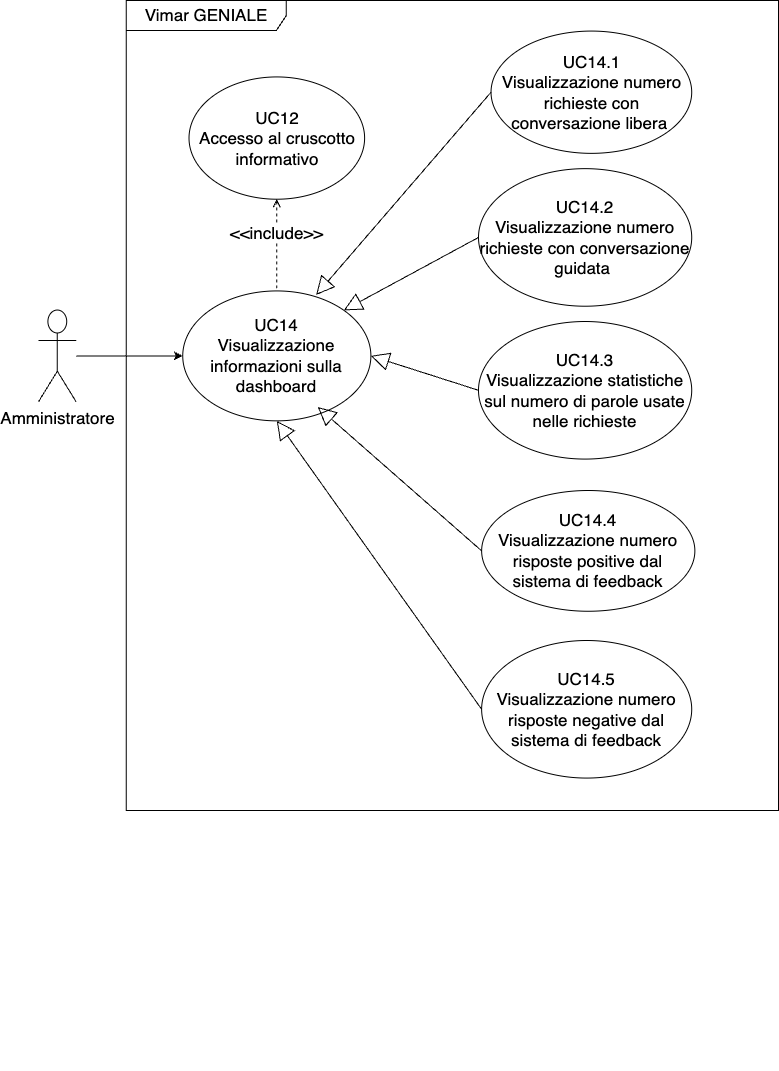
\includegraphics[width=0.8\textwidth]{contents/casi_duso/png/UC14.png}
\caption{UC14, UC14.1, UC14.2, UC14.3, UC14.4, UC14.5 - Visualizzazione informazioni \textit{dashboard}\textsubscript{G}}
% \label{fig:UC1a}
\end{figure}

\subuc{Visualizzazione numero richieste con \textit{conversazione libera}\textsubscript{G}}{visualizzazione_richieste_libere}
\begin{itemize}
    \item \textbf{Attori coinvolti}: \textit{Amministratore}\textsubscript{G};
    \item \textbf{Descrizione}: Un \textit{amministratore}\textsubscript{G} desidera visualizzare dal \textit{cruscotto informativo}\textsubscript{G} il numero delle richieste effettuate con una \textit{conversazione libera}\textsubscript{G};
    \item \textbf{Precondizioni}: 
        \begin{itemize}
            \item L’\textit{amministratore}\textsubscript{G} ha accesso all’\textit{interfaccia web}\textsubscript{G} del \textit{sistema}\textsubscript{G};
            \item L’\textit{amministratore}\textsubscript{G} è dotato dell’accesso alla \textit{dashboard}\textsubscript{G};
        \end{itemize}
    \item \textbf{Postcondizioni}: Il \textit{sistema}\textsubscript{G} raccoglie le informazioni relative al numero delle richieste effettuate con una \textit{conversazione libera}\textsubscript{G} e le mostra nella \textit{dashboard}\textsubscript{G};
    \item \textbf{Scenario principale}:
    \begin{enumerate}
    \item L’\textit{amministratore}\textsubscript{G} accede all’\textit{interfaccia web}\textsubscript{G} di Vimar GENIALE;
    \item Inserisce le proprie credenziali;
    \item Il \textit{sistema}\textsubscript{G} riceve la richiesta di accesso e \textit{verifica}\textsubscript{G} le credenziali;
    \item L’\textit{amministratore}\textsubscript{G} ottiene l’accesso alla \textit{dashboard}\textsubscript{G};
    \item Il \textit{sistema}\textsubscript{G} mostra le informazioni richieste sul \textit{cruscotto informativo}\textsubscript{G}.
    \end{enumerate}
\end{itemize}

\subuc{Visualizzazione numero richieste con \textit{conversazione guidata}\textsubscript{G}}{visualizzazione_richieste_guidate}
\begin{itemize}
    \item \textbf{Attori coinvolti}: \textit{Amministratore}\textsubscript{G};
    \item \textbf{Descrizione}: Un \textit{amministratore}\textsubscript{G} desidera visualizzare dal \textit{cruscotto informativo}\textsubscript{G} il numero delle richieste effettuate con una \textit{conversazione guidata}\textsubscript{G};
    \item \textbf{Precondizioni}: 
        \begin{itemize}
            \item L’\textit{amministratore}\textsubscript{G} ha accesso all’\textit{interfaccia web}\textsubscript{G} del \textit{sistema}\textsubscript{G};
            \item L’\textit{amministratore}\textsubscript{G} è dotato dell’accesso alla \textit{dashboard}\textsubscript{G};
        \end{itemize}
    \item \textbf{Postcondizioni}: Il \textit{sistema}\textsubscript{G} raccoglie le informazioni relative al numero delle richieste effettuate con una \textit{conversazione guidata}\textsubscript{G} e le mostra nella \textit{dashboard}\textsubscript{G};
    \item \textbf{Scenario principale}:
    \begin{enumerate}
    \item L’\textit{amministratore}\textsubscript{G} accede all’\textit{interfaccia web}\textsubscript{G} di Vimar GENIALE;
    \item Inserisce le proprie credenziali;
    \item Il \textit{sistema}\textsubscript{G} riceve la richiesta di accesso e \textit{verifica}\textsubscript{G} le credenziali;
    \item L’\textit{amministratore}\textsubscript{G} ottiene l’accesso alla \textit{dashboard}\textsubscript{G};
    \item Il \textit{sistema}\textsubscript{G} mostra le informazioni richieste sul \textit{cruscotto informativo}\textsubscript{G}.
    \end{enumerate}
\end{itemize}

\subuc{Visualizzazione classifica di parole più utilizzate}{visualizzazione_statistiche_parole}
\begin{itemize}
    \item \textbf{Attori coinvolti}: \textit{Amministratore}\textsubscript{G};
    \item \textbf{Descrizione}: Un \textit{amministratore}\textsubscript{G} desidera visualizzare dal \textit{cruscotto informativo}\textsubscript{G} la classifica delle parole più utilizzate con relativa percentuale rispetto al numero totale delle parole utilizzate nelle richieste;
    \item \textbf{Precondizioni}: 
        \begin{itemize}
            \item L’\textit{amministratore}\textsubscript{G} ha accesso all’\textit{interfaccia web}\textsubscript{G} del \textit{sistema}\textsubscript{G};
            \item L’\textit{amministratore}\textsubscript{G} è dotato dell’accesso alla \textit{dashboard}\textsubscript{G};
        \end{itemize}
    \item \textbf{Postcondizioni}: Il \textit{sistema}\textsubscript{G} raccoglie le informazioni relative alla classifica delle parole più utilizzate nelle richieste e la mostra nella \textit{dashboard}\textsubscript{G};
    \item \textbf{Scenario principale}:
    \begin{enumerate}
    \item L’\textit{amministratore}\textsubscript{G} accede all’\textit{interfaccia web}\textsubscript{G} di Vimar GENIALE;
    \item Inserisce le proprie credenziali;
    \item Il \textit{sistema}\textsubscript{G} riceve la richiesta di accesso e \textit{verifica}\textsubscript{G} le credenziali;
    \item L’\textit{amministratore}\textsubscript{G} ottiene l’accesso alla \textit{dashboard}\textsubscript{G};
    \item Il \textit{sistema}\textsubscript{G} mostra le informazioni richieste sul \textit{cruscotto informativo}\textsubscript{G}.
    \end{enumerate}
\end{itemize}

\subuc{Visualizzazione numero risposte positive dal \textit{sistema}\textsubscript{G} di \textit{feedback}\textsubscript{G}}{visualizzazione_risposte_positive}
\begin{itemize}
    \item \textbf{Attori coinvolti}: \textit{Amministratore}\textsubscript{G};
    \item \textbf{Descrizione}: Un \textit{amministratore}\textsubscript{G} desidera visualizzare dal \textit{cruscotto informativo}\textsubscript{G} il numero delle risposte positive dal \textit{sistema}\textsubscript{G} di \textit{feedback}\textsubscript{G};
    \item \textbf{Precondizioni}: 
        \begin{itemize}
            \item L’\textit{amministratore}\textsubscript{G} ha accesso all’\textit{interfaccia web}\textsubscript{G} del \textit{sistema}\textsubscript{G};
            \item L’\textit{amministratore}\textsubscript{G} è dotato dell’accesso alla \textit{dashboard}\textsubscript{G};
        \end{itemize}
    \item \textbf{Postcondizioni}: Il \textit{sistema}\textsubscript{G} raccoglie le informazioni relative al numero delle risposte positive dal \textit{sistema}\textsubscript{G} di \textit{feedback}\textsubscript{G} e le mostra nella \textit{dashboard}\textsubscript{G};
    \item \textbf{Scenario principale}:
    \begin{enumerate}
    \item L’\textit{amministratore}\textsubscript{G} accede all’\textit{interfaccia web}\textsubscript{G} di Vimar GENIALE;
    \item Inserisce le proprie credenziali;
    \item Il \textit{sistema}\textsubscript{G} riceve la richiesta di accesso e \textit{verifica}\textsubscript{G} le credenziali;
    \item L’\textit{amministratore}\textsubscript{G} ottiene l’accesso alla \textit{dashboard}\textsubscript{G};
    \item Il \textit{sistema}\textsubscript{G} mostra le informazioni richieste sul \textit{cruscotto informativo}\textsubscript{G}.
    \end{enumerate}
\end{itemize}

\subuc{Visualizzazione numero risposte negative dal \textit{sistema}\textsubscript{G} di \textit{feedback}\textsubscript{G}}{visualizzazione_risposte_negative}
\begin{itemize}
    \item \textbf{Attori coinvolti}: \textit{Amministratore}\textsubscript{G};
    \item \textbf{Descrizione}: Un \textit{amministratore}\textsubscript{G} desidera visualizzare dal \textit{cruscotto informativo}\textsubscript{G} il numero delle risposte negative dal \textit{sistema}\textsubscript{G} di \textit{feedback}\textsubscript{G};
    \item \textbf{Precondizioni}: 
        \begin{itemize}
            \item L’\textit{amministratore}\textsubscript{G} ha accesso all’\textit{interfaccia web}\textsubscript{G} del \textit{sistema}\textsubscript{G};
            \item L’\textit{amministratore}\textsubscript{G} è dotato dell’accesso alla \textit{dashboard}\textsubscript{G};
        \end{itemize}
    \item \textbf{Postcondizioni}: Il \textit{sistema}\textsubscript{G} raccoglie le informazioni relative al numero delle risposte negative dal \textit{sistema}\textsubscript{G} di \textit{feedback}\textsubscript{G} e le mostra nella \textit{dashboard}\textsubscript{G};
    \item \textbf{Scenario principale}:
    \begin{enumerate}
    \item L’\textit{amministratore}\textsubscript{G} accede all’\textit{interfaccia web}\textsubscript{G} di Vimar GENIALE;
    \item Inserisce le proprie credenziali;
    \item Il \textit{sistema}\textsubscript{G} riceve la richiesta di accesso e \textit{verifica}\textsubscript{G} le credenziali;
    \item L’\textit{amministratore}\textsubscript{G} ottiene l’accesso alla \textit{dashboard}\textsubscript{G};
    \item Il \textit{sistema}\textsubscript{G} mostra le informazioni richieste sul \textit{cruscotto informativo}\textsubscript{G}.
    \end{enumerate}
\end{itemize}



\uc{Richiesta di argomento proibito}{argomento_proibito}
\begin{itemize}
    \item \textbf{Attori coinvolti}: Installatore;
    \item \textbf{Descrizione}: L’installatore richiede argomenti proibiti al \textit{sistema}\textsubscript{G} (e.g. politica, finanza, pornografia, ...);
    \item \textbf{Precondizioni}: 
        \begin{itemize}
            \item L’installatore ha accesso all’\textit{interfaccia web}\textsubscript{G} del \textit{sistema}\textsubscript{G};
            \item L’installatore ha accesso ad una conversazione memorizzabile nel \textit{sistema}\textsubscript{G};
            \item La domanda posta non riguarda argomenti proibiti.
        \end{itemize}
    \item \textbf{Postcondizioni}: Il \textit{sistema}\textsubscript{G} restituisce una risposta che indica il motivo per cui si è verificato l’errore;
    \item \textbf{Scenario principale}:
    \begin{enumerate}
    \item L’installatore accede all’\textit{interfaccia web}\textsubscript{G} di Vimar GENIALE;
    \item Inserisce una domanda inconsistente, che non ha a che vedere con prodotti \textit{VIMAR}\textsubscript{G};
    \item Il \textit{sistema}\textsubscript{G} elabora la richiesta e fornisce una risposta che spiega la causa dell'errore riscontrato;
    \item L’installatore visualizza le informazioni sull’errore che si è verificato;
    \end{enumerate}
     \item \textbf{Inclusioni}: UC6 - Ricerca informazioni sui prodotti con conversazione libera.
\end{itemize}

\uc{Domanda al sistema\textsubscript{G}}{domanda}
\begin{itemize}
    \item \textbf{Attori coinvolti}: Installatore;
    \item \textbf{Descrizione}: L’installatore inserisce una domanda;
    \item \textbf{Precondizioni}: 
        \begin{itemize}
            \item L’installatore ha accesso all’\textit{interfaccia web}\textsubscript{G} del \textit{sistema}\textsubscript{G};
            \item L’installatore ha accesso ad una conversazione memorizzabile nel \textit{sistema}\textsubscript{G};
            \item L'installatore ha inviato una domanda al \textit{sistema}\textsubscript{G};
            \item La domanda posta non riguarda argomenti proibiti.
        \end{itemize}
    \item \textbf{Postcondizioni}: Il \textit{sistema}\textsubscript{G} restituisce una risposta;
    \item \textbf{Scenario principale}:
    \begin{enumerate}
    \item L’installatore accede all’\textit{interfaccia web}\textsubscript{G} di Vimar GENIALE;
    \item Inserisce una domanda che ha a che vedere con prodotti \textit{VIMAR}\textsubscript{G} e non con argomenti proibiti o sconosciuti;
    \item Il \textit{sistema}\textsubscript{G} elabora la richiesta e fornisce una risposta;
    \item L’installatore visualizza le informazioni restituite;
    \end{enumerate}
\end{itemize}
\begin{figure}[H]
\centering
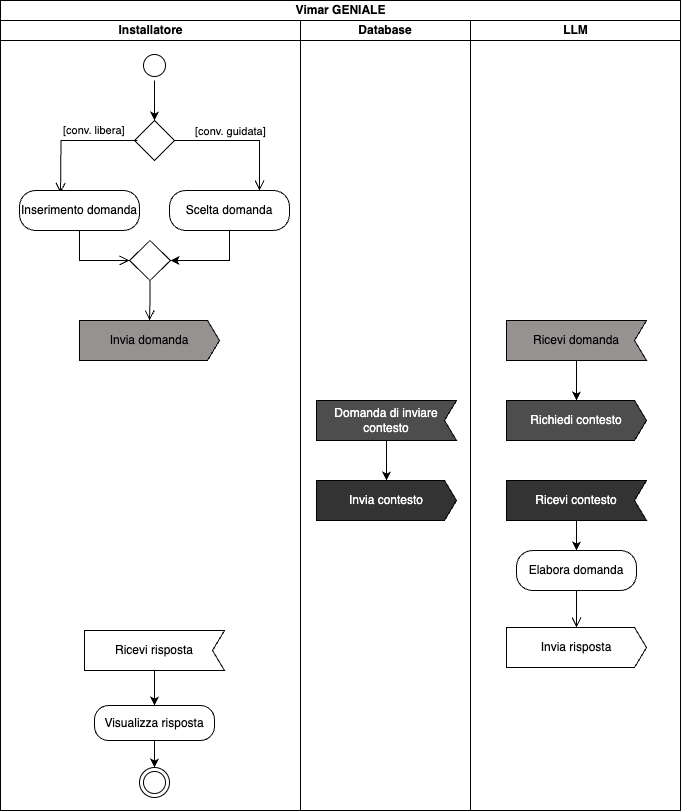
\includegraphics[width=0.8\textwidth]{contents/casi_duso/png/UC16_activity.png}
\caption{UC16 - Domanda al \textit{sistema}\textsubscript{G}}
% \label{fig:UC1a}
\end{figure}

\uc{Richiesta di uno schema o immagine}{domanda_immagine}
\begin{itemize}
    \item \textbf{Attori coinvolti}: Installatore;
    \item \textbf{Descrizione}: L’installatore inserisce una domanda la cui risposta prevede uno schema elettrico o un'immagine;
    \item \textbf{Precondizioni}: 
        \begin{itemize}
            \item L’installatore ha accesso all’\textit{interfaccia web}\textsubscript{G} del \textit{sistema}\textsubscript{G};
            \item L’installatore ha accesso ad una conversazione memorizzabile nel \textit{sistema}\textsubscript{G};
            \item L'installatore ha inviato una domanda al \textit{sistema}\textsubscript{G};
            \item La risposta alla domanda posta necessita, per essere completa, si uno schema elettrico o di un'immagine.
        \end{itemize}
    \item \textbf{Postcondizioni}: Il \textit{sistema}\textsubscript{G} restituisce una risposta con l'immagine o lo schema corretto;
    \item \textbf{Scenario principale}:
    \begin{enumerate}
    \item L’installatore accede all’\textit{interfaccia web}\textsubscript{G} di Vimar GENIALE;
    \item Inserisce una domanda che ha a che vedere con prodotti \textit{VIMAR}\textsubscript{G};
    \item Il \textit{sistema}\textsubscript{G} elabora la richiesta e fornisce una risposta inserendo uno schema o di un'immagine di cui la risposta ha bisogno per essere esaustiva;
    \item L’installatore visualizza le informazioni restituite;
    \end{enumerate}
    \item \textbf{Generalizzazioni}: UC6 - Ricerca informazioni sui prodotti con \textit{conversazione libera}\textsubscript{G}.  
\end{itemize}



\uc{ Digitazione della Domanda}{digita_domanda}
\begin{itemize}
    \item \textbf{Attori coinvolti}: Installatore;
    \item \textbf{Descrizione}: L’installatore inserisce una domanda;
    \item \textbf{Precondizioni}: 
        \begin{itemize}
            \item L’installatore ha accesso all’\textit{interfaccia web}\textsubscript{G} del \textit{sistema}\textsubscript{G};
        \end{itemize}
    \item \textbf{Postcondizioni}: L'installatore invia la domanda al \textit{sistema}\textsubscript{G};
    \item \textbf{Scenario principale}:
    \begin{enumerate}
    \item L’installatore accede all’\textit{interfaccia web}\textsubscript{G} di Vimar GENIALE;
    \item Inserisce una domanda;
    \item Il \textit{sistema}\textsubscript{G} riceve la domanda ed inizia ad elaborarla;
    \end{enumerate}
    \item \textbf{Estensioni}: UC7 - Superamento limite caratteri del messaggio.
\end{itemize}

\uc{Visualizzazione singolo messaggio}{visualizza_messaggio}
\begin{itemize}
    \item \textbf{Attori coinvolti}: Installatore;
    \item \textbf{Descrizione}: L'installatore visualizza il singolo messaggio;
    \item \textbf{Precondizioni}: 
        \begin{itemize}
            \item L'installatore ha creato una conversazione e ha inviato (o ricevuto) un messaggio;
        \end{itemize}
    \item \textbf{Postcondizioni}: 
    \begin{enumerate}
        \item L'installatore visualizza il singolo messaggio;
    \end{enumerate}
    \item \textbf{Scenario principale}:
    \begin{enumerate}
        \item L'installatore invia o riceve un messaggio da Vimar GENIALE;
        \item l'installatore visualizza il mesaggio;
    \end{enumerate}
    \item \textbf{Estensioni}: UC9 - Visualizzazione storico dei messaggi.
    \item \textbf{Inclusioni}: 
    \begin{itemize}
        \item UC19.1 - Visualizzazione data invio del messaggio;
        \item UC19.2 - Visualizzazione ora invio del messaggio.
    \end{itemize}
\end{itemize}
\begin{figure}[H]
\centering
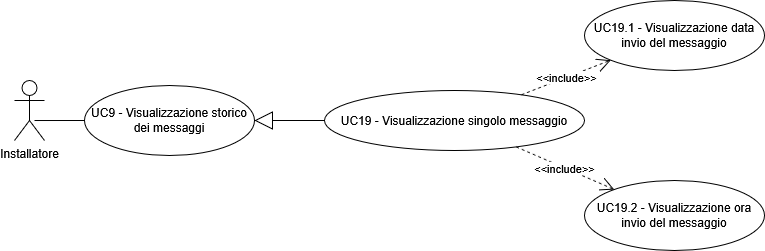
\includegraphics[width=0.8\textwidth]{contents/casi_duso/png/UC19.png}
\caption{UC16 - Domanda al \textit{sistema}\textsubscript{G}}
% \label{fig:UC1a}
\end{figure}

\subuc{Visualizzazione data invio del messaggio}{visualizza_data}
\begin{itemize}
    \item \textbf{Attori coinvolti}: Installatore;
    \item \textbf{Descrizione}: L'installatore visualizza la data di invio del messaggio;
    \item \textbf{Precondizioni}:  
        \begin{itemize}
            \item L'installatore ha creato una conversazione e ha inviato (o ricevuto) un messaggio;
        \end{itemize}
    \begin{enumerate}
        \item L'installatore visualizza la data di invio del messaggio;
    \end{enumerate}
    \item \textbf{Scenario principale}:
    \begin{enumerate}
        \item L'installatore invia o riceve un messaggio da Vimar GENIALE;
        \item l'installatore visualizza la data di invio del messaggio;
    \end{enumerate}
\end{itemize}

\subuc{Visualizzazione orario invio del messaggio}{visualizza_ora}
\begin{itemize}
    \item \textbf{Attori coinvolti}: Installatore;
    \item \textbf{Descrizione}: L'installatore visualizza l'ora di invio del messaggio;
    \item \textbf{Precondizioni}:  
        \begin{itemize}
            \item L'installatore ha creato una conversazione e ha inviato (o ricevuto) un messaggio;
        \end{itemize}
    \begin{enumerate}
        \item L'installatore visualizza l'ora di invio del messaggio;
    \end{enumerate}
    \item \textbf{Scenario principale}:
    \begin{enumerate}
        \item L'installatore invia o riceve un messaggio da Vimar GENIALE;
        \item l'installatore visualizza l'ora di invio del messaggio;
    \end{enumerate}
\end{itemize}

